\documentclass{article}

\usepackage{amsmath}
\usepackage[margin=0.75in]{geometry}
\usepackage{graphicx}
\usepackage{hyperref}
\hypersetup{
	linkcolor=blue,
	colorlinks=true
}
\usepackage{blkarray}
\usepackage{caption}


\title{The theory and implementation of kCON}

\author{Xin Chen}
\date{\today}


\begin{document}
\maketitle


\section{Overview}

kCON is scalable and transferable deep learning framework for chemistry with the ability to 
provide insight into atomistic structures of varying stoichiometry from small and scrap 
training sets. kCON is built upon convolutional neural networks, or more specifically, 
1D-convolutional neural networks with 1x1 convolutions.

%\begin{center}
%  \makebox[\textwidth]{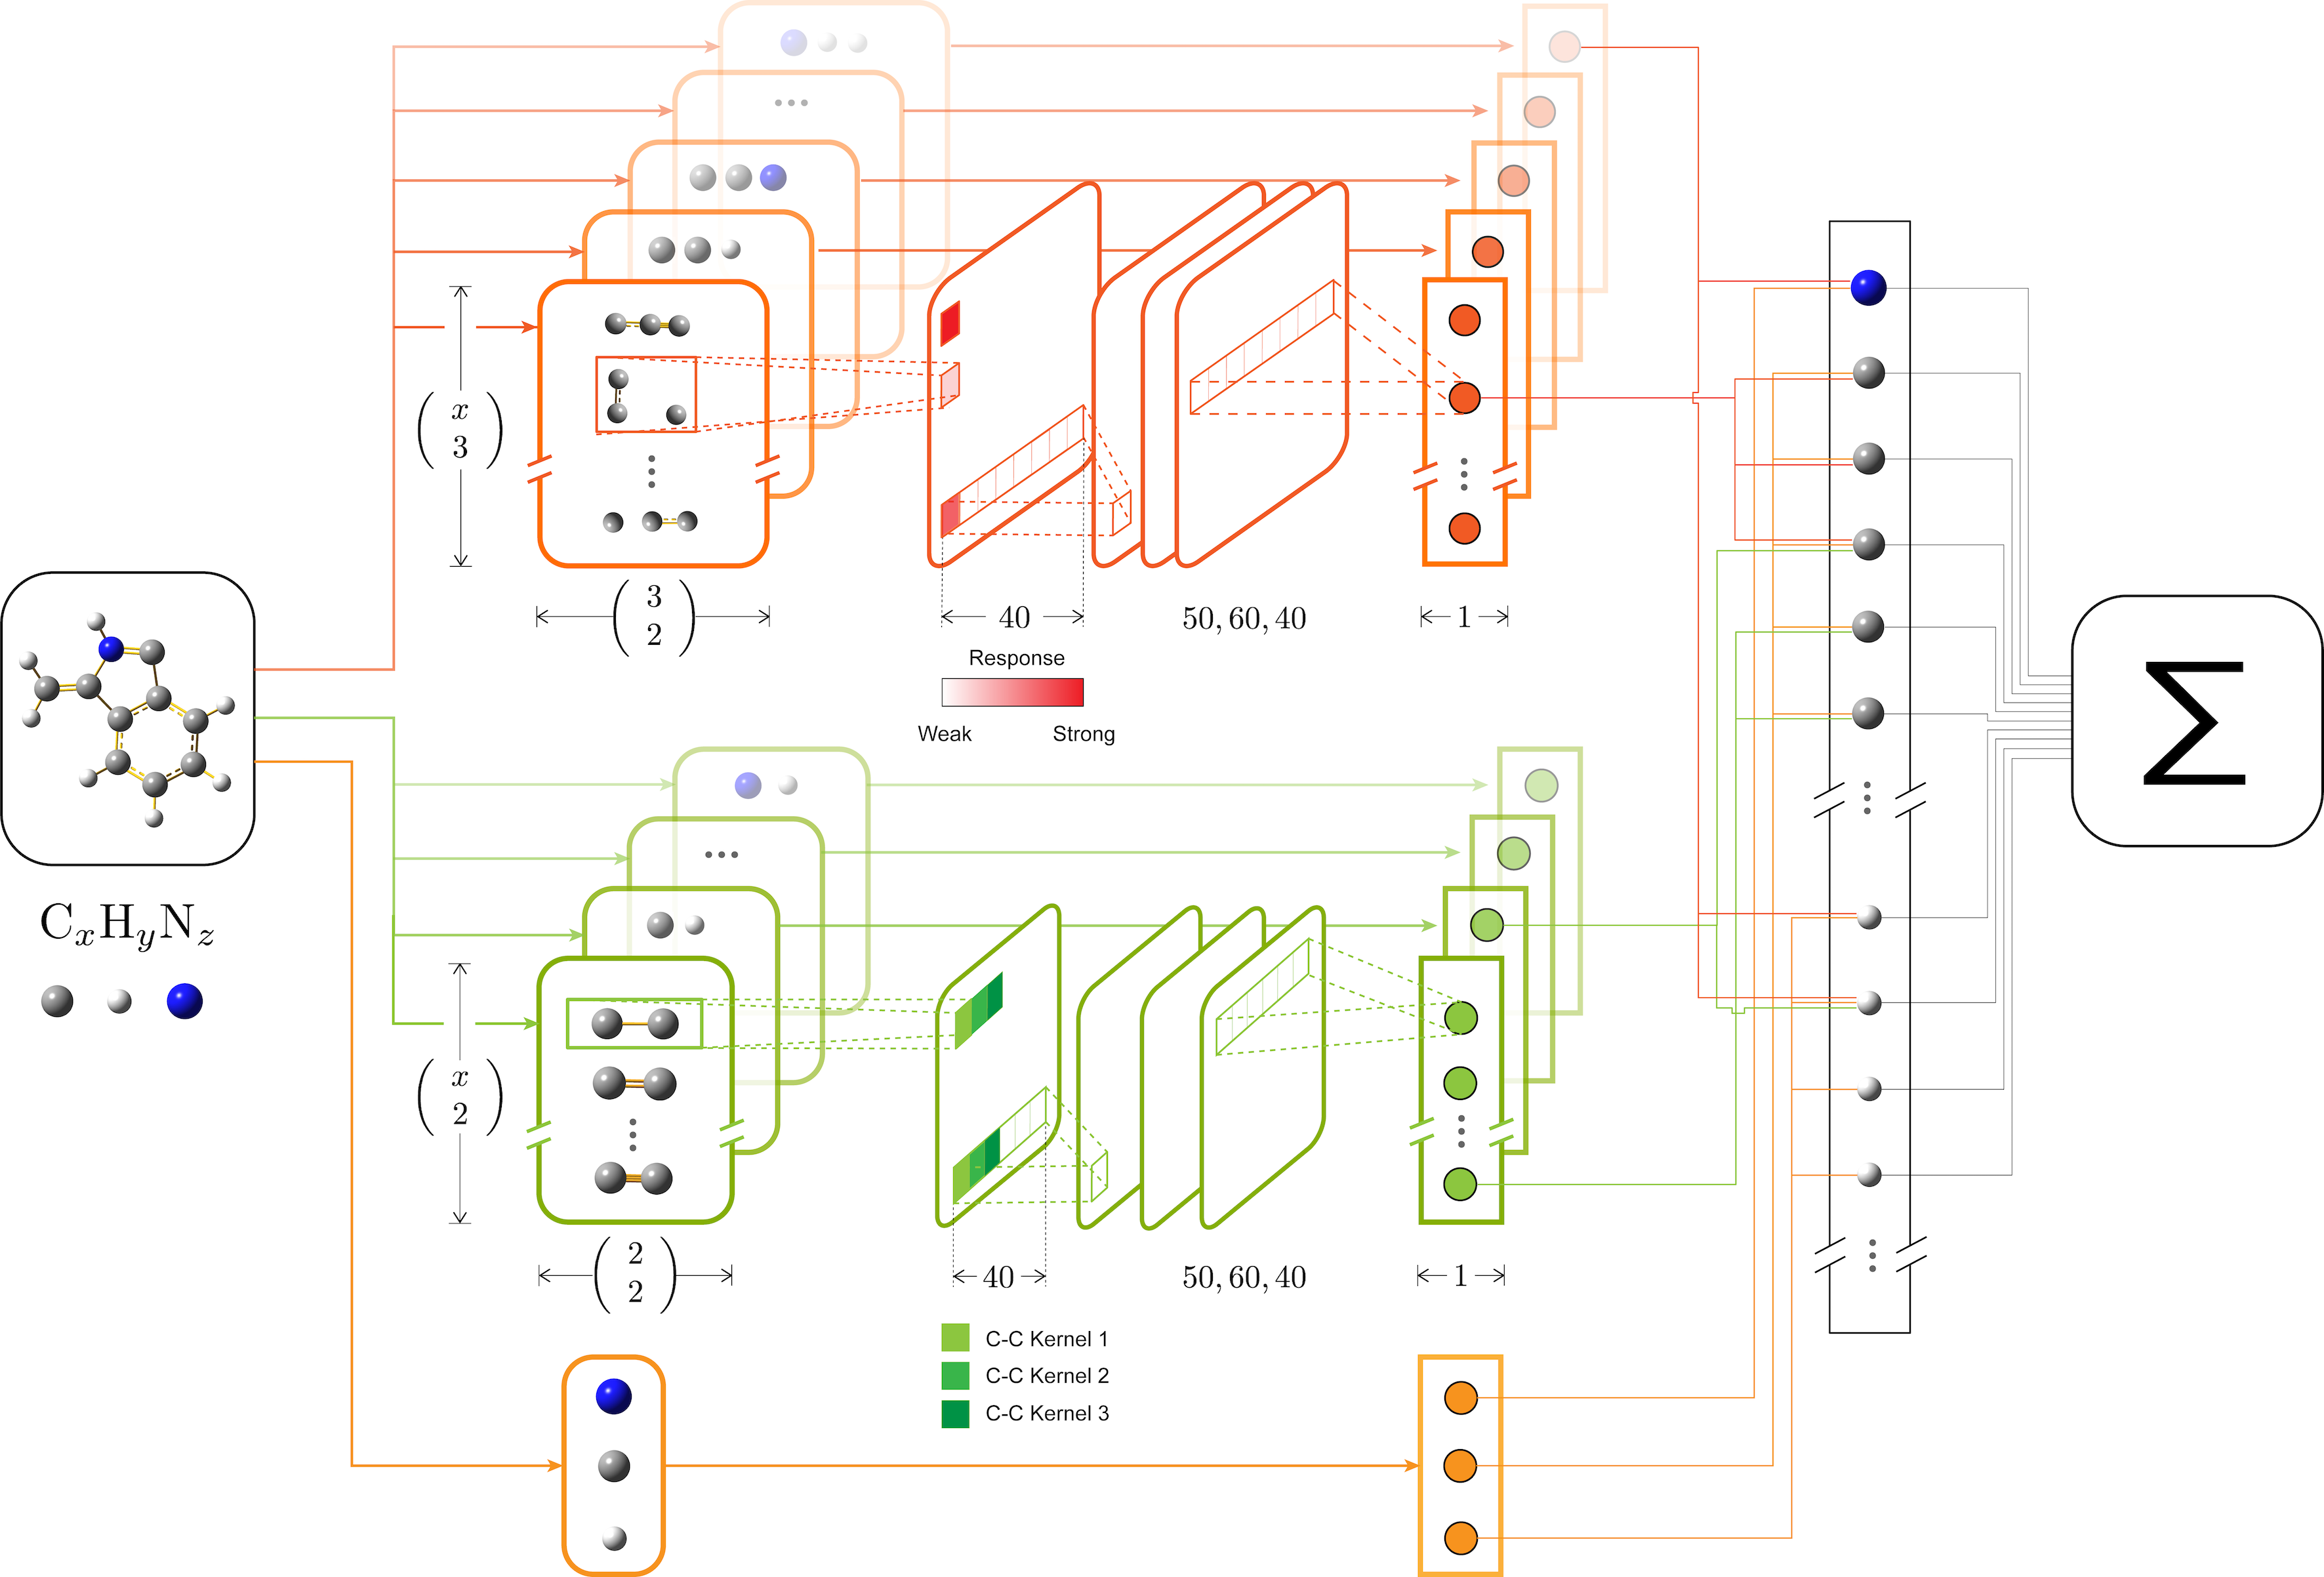
\includegraphics[width=0.8\paperwidth]{images/figure1}}
%\end{center}

\section{Energy}

The total energy output by kCON is modeled under the many-body expression scheme:

\begin{eqnarray}\label{MBE}
E^{total}
& = &
E^{(k=1)} + E^{(k=2)} + E^{(k=3)} + \cdots \nonumber \\
& = & 
\sum_{a}^{C^N_1}{E^{(k=1)}_{a}} + 
\sum_{a,b}^{C^{N}_2}{E^{(k=2)}_{ab}} + 
\sum_{a,b,c}^{C^{N}_3}{E^{(k=3)}_{abc}} + \cdots \nonumber \\
& = & 
\sum_{a}^{C^N_1}{\mathbf{F}^{(k=1)}(A_a)} + 
\sum_{a,b}^{C^{N}_2}{\mathbf{F}^{(k=2)}(r_{ab}, A_a, A_b)} + 
\sum_{a,b,c}^{C^{N}_3}{\mathbf{F}^{(k=3)}(r_{ab}, r_{bc}, r_{ac}, A_a, A_b, A_c)} + \cdots
\end{eqnarray}

\noindent where $r_{ab}$ denotes the interatomic distance between atom $a$ and $b$, $A_A$ 
represents the element of atom $a$, $\mathbf{F}^{(k)}$ is an arbitrary function that outputs
the energy for k-body inputs.

For most cases, equation \ref{MBE} can be truncated at $k = 3$ because 
higher order terms contribute far less to the total energy while require much more 
computational resources as $C^N_k$ roughly scales as $\mathcal{O}(N)$ and the 2-body 
features alone (bonds) cannot uniquely describe structures. The interatomic distances, 
${r_{ab}}$, range from 0 to $+\infty$. To normalize the distances, the Laplacian kernel is 
used:

\begin{eqnarray}\label{eqn:laplacian}
z_{ab} 
= \exp{\left(-\frac{r_{ab}}{L_{a} + L_{b}}\right)}
= \exp{\left(-\frac{r_{ab}}{L_{ab}}\right)}
\end{eqnarray}

\noindent where $L_{a}$ is the covalent radius of element $A_{a}$. For non periodic 
molecules the \href{http://pubs.acs.org/doi/pdf/10.1021/jp5065819}
{P$\ddot{\mathrm{y}}\ddot{\mathrm{y}}$kko radii} are used as the covalent radii and 
for periodic structures the 
\href{http://pubs.rsc.org/en/content/articlepdf/2008/DT/B801115J}{CSD covalent bonds} should be 
used. 

Then the MBE expression becomes:

\begin{eqnarray}\label{eqn:total_energy}
E^{total} =
\sum_{a}^{C^N_1}{\mathbf{F}^{(k=1)}(A_a)} + 
\sum_{a,b}^{C^{N}_2}{\mathbf{F}^{(k=2)}(z_{ab}, A_a, A_b)} + 
\sum_{a,b,c}^{C^{N}_3}{\mathbf{F}^{(k=3)}(z_{ab}, z_{bc}, z_{ac}, A_a, A_b, A_c)}
\end{eqnarray}

\noindent Now what we need is to model the three $\mathbf{F}^{(k)}$.

\subsection{One-body}

In kCON, the 1-body terms are expressed by a linear model:

\begin{eqnarray}
\mathbf{F}^{(k=1)}(A_a) 
& = & 
E^{A_a} \\
\sum_{a}^{C^N_1}{\mathbf{F}^{(k=1)}(A_a)} 
& = & 
\sum_{a}^{N}{E^{A_a}} = \sum_{A_{a}}{n^{A_a}E^{A_a}}
\end{eqnarray}

\noindent where $E^{A_a}$ represents the learnable 1-body energy of element $A_a$ and 
$n^{A_a}$ is the total number of element $A_a$ in the structure. As an example, the 1-body 
energy of a $\mathrm{C}_9 \mathrm{H}_7 \mathrm{N}$ molecule should be:

\begin{eqnarray}
E^{(k=1)} = 9E^{\mathrm{C}} + 7E^{\mathrm{H}} + E^{\mathrm{N}}
\end{eqnarray}

\noindent where $E^{\mathrm{C}}$, $E^{\mathrm{H}}$ and $E^{\mathrm{N}}$ are all trainable 
parameters.

The reason to use a simple linear model to express the 1-body term is that we observed that for 
chemically reasonable structures, for example the organic compounds in QM7 and GDB-9 datasets 
that can be synthesized, even the linear model can give acceptable energy predictions.

\begin{center}
\makebox[\textwidth]{
	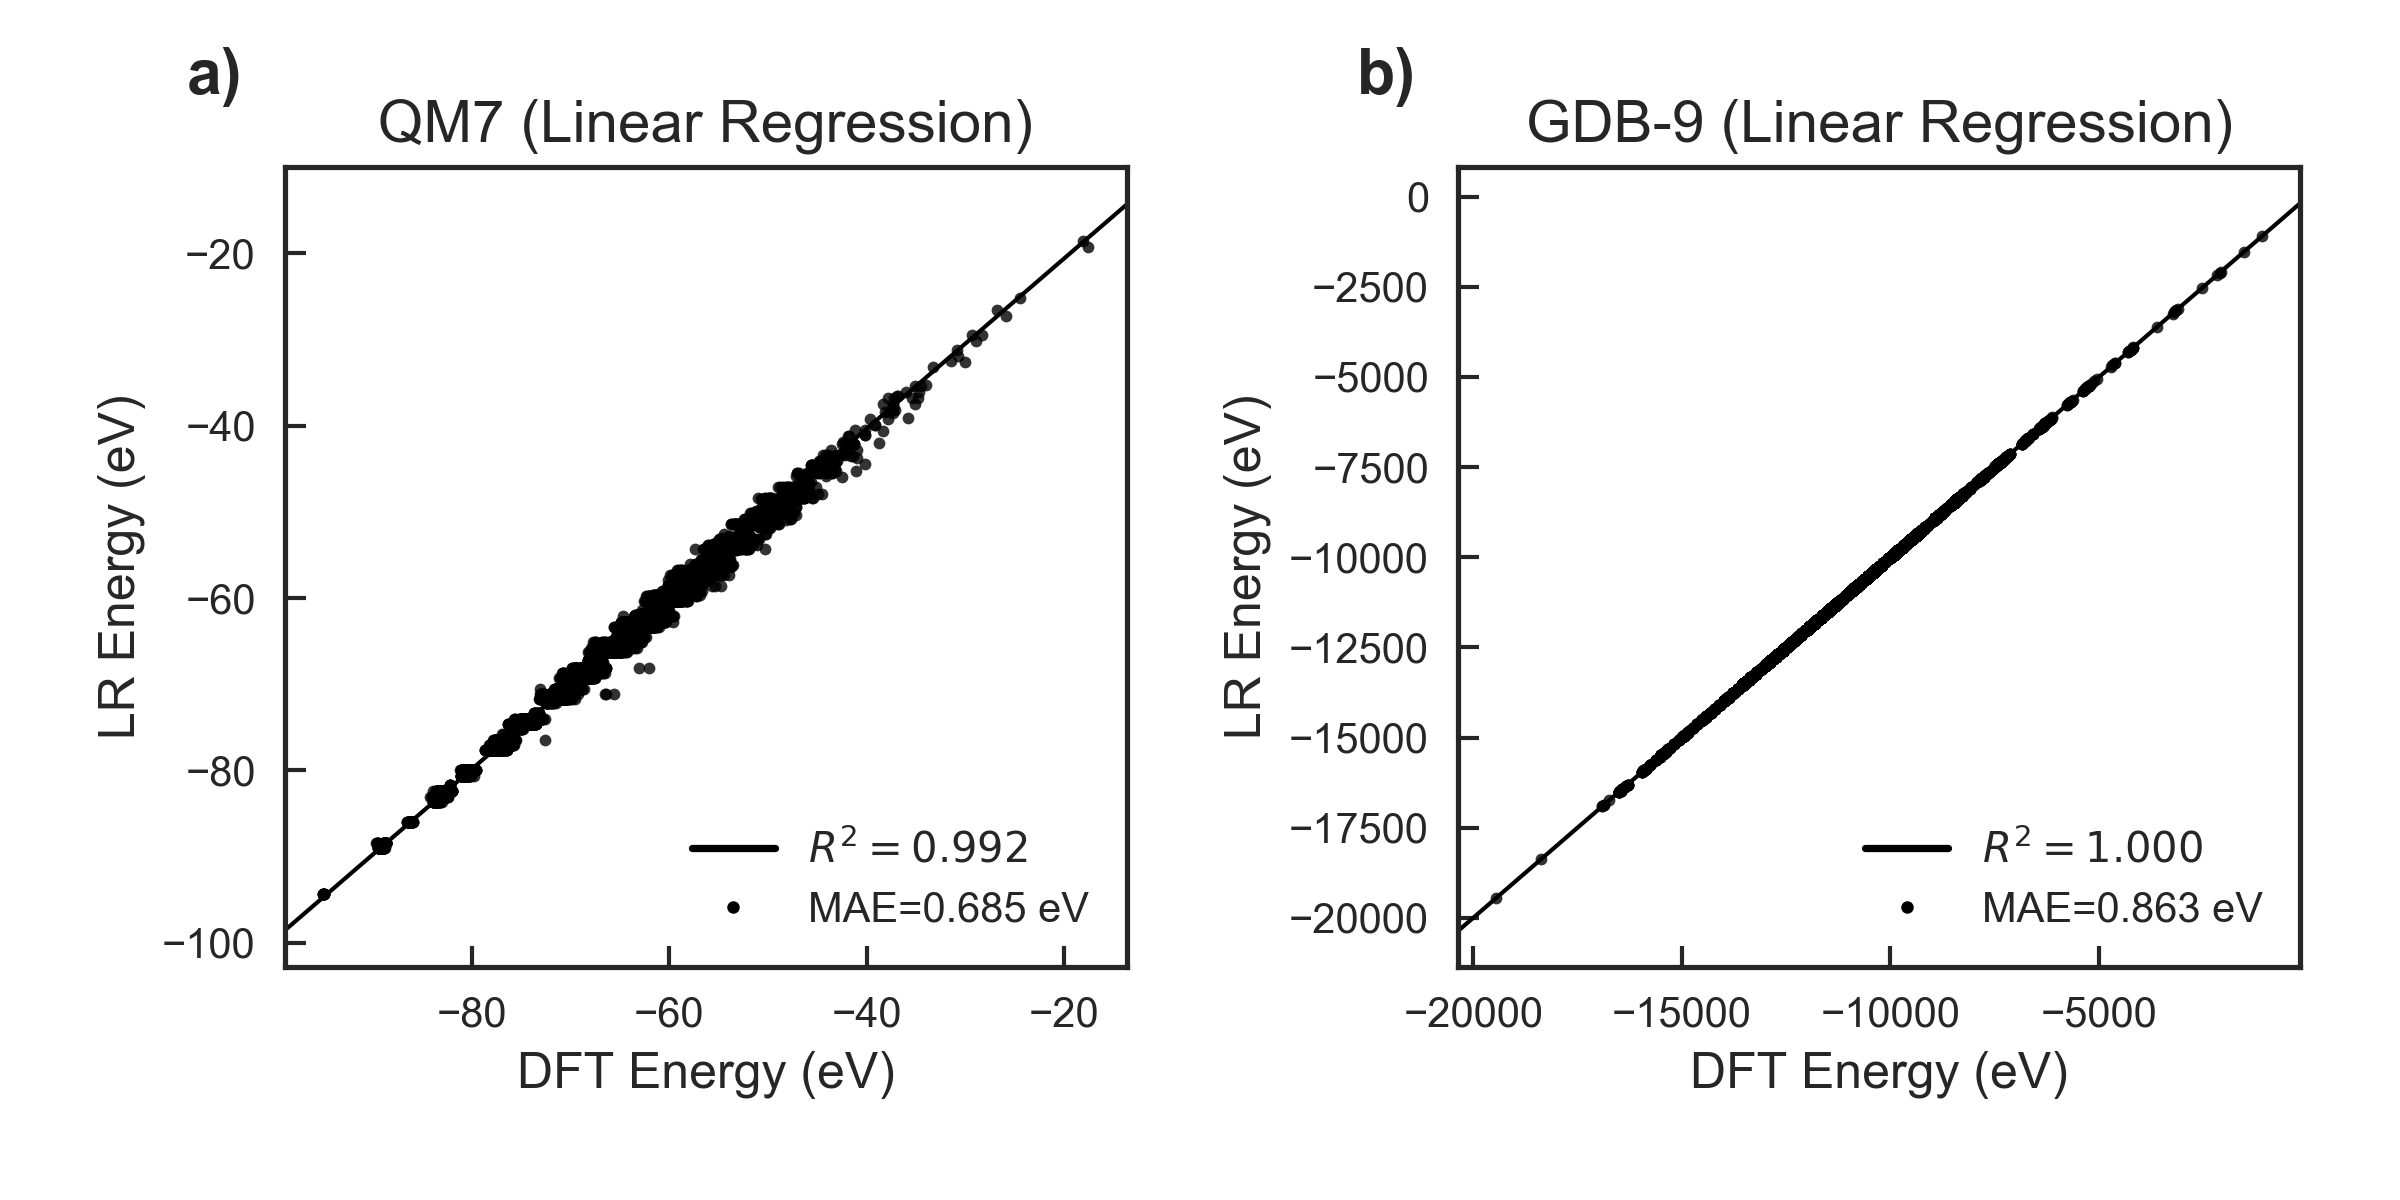
\includegraphics[width=0.6\paperwidth]{images/figureS2}
}
\end{center}

\subsection{Two/three-body}

Modeling the 2-body and 3-body interactions are more complicated because if we want our model 
transferable, the model must support accepting variable-length inputs so that a single model 
can be used to process atomistic structures of varying size and composition. 

So here, we use 1D-convolutional neural networks to model $\mathbf{F}^{(k=2)}$ and 
$\mathbf{F}^{(k=2)}$. For each k-body term (k-body interactions, e.g. Carbon-Carbon-Carbon),
an independent CNN is used. So kCON is indeed a model composed of a collection of k-body CNNs 
and a linear model.

\begin{eqnarray}
E^{(k=2)} & = & \sum_{a,b}^{C^N_2}{
	\boldmath{\mathrm{CNN}}^{\mathrm{A}_{a}\mathrm{A}_{b}}
}(r_{ab}) \\
\label{eqn:cnn_f_3}
E^{(k=3)} & = & \sum_{a,b,c}^{C^N_3}{
	\boldmath{\mathrm{CNN}}^{\mathrm{A}_{a}\mathrm{A}_{b}\mathrm{A}_{c}}
}(r_{ab}, r_{ac}, r_{bc})
\end{eqnarray}

\noindent As an example, the $\mathrm{C}_9 \mathrm{H}_7 \mathrm{N}$ system has five 2-body 
terms (CC, CH, CN, HH, HN) and seven 3-body terms (CCC, CCH, CCN, CHH, CHN, HHH, HHN). So the 
kCON model for $\mathrm{C}_9 \mathrm{H}_7 \mathrm{N}$ has 12 independent CNNs to train at the 
same time.

The activation function $\sigma(\cdot)$ used in kCON is leaky ReLU:

\begin{eqnarray}\label{eqn:lrelu}
\sigma(x) & = & \begin{cases}
	x & \quad \text{if } x \geq 0 \\
	\alpha x & \quad \text{else} \\
\end{cases} \\
\frac{\partial{\sigma(x)}}{\partial{x}} & = & \begin{cases}
	1 & \quad \text{if } x \geq 0 \\
	\alpha & \quad \text{else} \\
\end{cases} \\
\alpha & = & 0.2
\end{eqnarray}

\noindent because leaky ReLU can give much better results compared with traditional activations 
functions like hyperbolic tangent (tanh) or sigmoid.

\subsection{The input feature matrix}

Now we can start building the inputs for kCON. Inputs for the 1-body part is very simple, so 
here we mainly focus on how to efficiently build input feature matrix for 2-body and 3-body 
terms.

As introduced before, kCON has a collection of k-body CNNs. But for any specific chemical 
system, the dimensions of its k-body terms should be fixed. For example, table \ref{tab:table1}
demonstrates the sizes of the k-body terms of the $\mathrm{C}_9 \mathrm{H}_7 \mathrm{N}$ 
system:

\begin{table}[h]
	\center
	\begin{tabular}{l*{3}{c}r}
		Term              & k & Expression & Dimension \\
		\hline
		CC    & 2 & $C^9_2$                         &  36 \\
		CH    & 2 & $C^9_1 \cdot C^7_1$             &  63 \\
		CN    & 2 & $C^9_1 \cdot C^1_1$             &   9 \\
		HH    & 2 & $C^7_2$                         &  21 \\
		HN    & 2 & $C^7_1 \cdot C^1_1$             &   7 \\
		CCC   & 3 & $C^9_3$                         &  84 \\
		CCH   & 3 & $C^9_2 \cdot C^7_1$             & 252 \\
		CCN   & 3 & $C^9_2 \cdot C^1_1$             &  36 \\
		CHH   & 3 & $C^9_1 \cdot C^7_2$             & 189 \\
		CHN   & 3 & $C^9_1 \cdot C^7_1 \cdot C^1_1$ &  63 \\
		HHH   & 3 & $C^7_3$                         &  35 \\
		HHN   & 3 & $C^7_2 \cdot C^1_1$             &  21 \\
		Total &   &                                 & 816
	\end{tabular}
	\caption{
		the dimensions of the k-body terms of $\mathrm{C}_9 \mathrm{H}_7 \mathrm{N}$
	}
	\label{tab:table1}
\end{table}

\noindent Instead of generating separated inputs for each k-body CNN, we can build a single input 
matrix and split it based on the dimensions. For a system composed of N atoms, the total number
of input patterns should be:

\begin{equation}\label{eqn:cn3_cn2}
C^N_3 + C^N_2 = C^{N+1}_3
\end{equation}

\noindent and the total number of entries (element in the input feature matrix) should be:

\begin{equation}
C^N_3 \cdot C^3_2 + C^N_2 \cdot C^1_1 = \frac{N(N-1)^2}{2}
\end{equation}

One can notice that for a system with N atoms the number of chemical patterns is $C^{N+1}_3$.
So a more easy way can be used to construct the input feature matrix. This scheme is called
\textbf{ghost atom scheme}. We can just temporarily append a ghost atom, denoted as 
\textbf{X}, to the original system and only keep the 3-body features. 
The cartesian coordinates of the ghost atom is always $(+\infty, +\infty, +\infty)$, 
so the interatomic distance between X and any real atom is $+\infty$. Thus, the Laplacian 
normalization, defined in equation \ref{eqn:laplacian}, will transform all distances between 
\textbf{X} and real atoms to 0. 

As an example shown, table \ref{tab:table2} shows the 
dimensions of the 3-body terms of the $\mathrm{C}_9 \mathrm{H}_7 \mathrm{N}X$ system: 
\begin{table}[h]
	\center
	\begin{tabular}{l*{3}{c}r}
		Term              & k & Expression & Dimension \\
		\hline
		CCX   & 3 & $C^9_2 \cdot C^1_1$             &  36 \\
		CHX   & 3 & $C^9_1 \cdot C^7_1 \cdot C^1_1$ &  63 \\
		CNX   & 3 & $C^9_1 \cdot C^1_1 \cdot C^1_1$ &   9 \\
		HHX   & 3 & $C^7_2 \cdot C^1_1$             &  21 \\
		HNX   & 3 & $C^7_1 \cdot C^1_1 \cdot C^1_1$ &   7 \\
		CCC   & 3 & $C^9_3$                         &  84 \\
		CCH   & 3 & $C^9_2 \cdot C^7_1$             & 252 \\
		CCN   & 3 & $C^9_2 \cdot C^1_1$             &  36 \\
		CHH   & 3 & $C^9_1 \cdot C^7_2$             & 189 \\
		CHN   & 3 & $C^9_1 \cdot C^7_1 \cdot C^1_1$ &  63 \\
		HHH   & 3 & $C^7_3$                         &  35 \\
		HHN   & 3 & $C^7_2 \cdot C^1_1$             &  21 \\
		Total &   &                                 & 816 
	\end{tabular}	
	\caption{
		the dimensions of the k-body terms of $\mathrm{C}_9 \mathrm{H}_7 \mathrm{N}X$
	}
	\label{tab:table2}
\end{table}

\noindent We can notice that the total number of input chemical patterns is unchanged. The 
total number of entries becomes:

\begin{equation}
C^{N+1}_3 \cdot C^3_2 = \frac{N(N-1)^2}{2} + C^N_2 \cdot 2
\end{equation}

\noindent so we need more space to store the input features but this is worthy as all features 
can be saved in a single matrix of shape $[C^{N+1}_3, C^3_2]$.

\subsection{Permutational Invariance}

The three spatial (translational, rotational and permutational) invariances must all be 
satisfied. Since kCON only uses interatomic distances $r$, the translational and 
rotational invariances are naturally kept and the 1-body and 2-body terms are also 
permutationally invariant. However, the 3-body terms cannot uphold this
requirement because the orders of the parameters of convolutional kernels are fixed 
while $(r_{ab}, r_{ac}, r_{bc})$ in equation \ref{eqn:cnn_f_3} must be inter-changeable.

To overcome this problem, the conditional sorting scheme is adopted: the columns of the 
input matrix (the input layer) of each k-body CNN are ordered according to the bond types, 
and for each k-body interaction (matrix row) we only sort the  entries of the same atom 
types. Taking the examples of CHN, CCH and CCC:

\begin{itemize}
	\item CHN: each column represents a unique bond type (C-H, C-N, H-N). Sorting is not needed.
	\item CCN: the entries corresponding to C-C of each row should be sorted.
	\item CCC: all three entries of each row should be sorted.
\end{itemize}

\subsection{Loss}

By default, kCON uses the root mean squared error as the total loss to minimize:

\begin{eqnarray}
\mathrm{RMSE} = \sqrt{
	\frac{1}{n}
	\sum_{i=1}^{n}{ 
		\left( E_{i}^{\mathrm{kCON}} - E_{i}^{\mathrm{True}} \right)^2
	}
}	
\end{eqnarray}

\noindent kCON also supports exponentially-scaled RMSE if the contributions of the unstable 
structures should be minimized:

\begin{eqnarray}
\mathrm{esRMSE} = \sqrt{
	\frac{1}{n} 
	\sum_{i=1}^{n}{
		\exp{\left(-\frac{E_{i}^{\mathrm{kCON}} - E_{i}^{\mathrm{True}}}{k_BT} \right)}
		\left(E_{i}^{\mathrm{kCON}} - E_{i}^{\mathrm{True}} \right)^2
	}
}	
\end{eqnarray}

\subsection{Atomic Energy}

The concept of atomic energy was first proposed by 
\href{https://journals.aps.org/prl/abstract/10.1103/PhysRevLett.98.146401}{Behler et al} in 
2007. Despite that many later machine learning models include the concept of atomic energy, 
very little work has been done on interpreting the chemical meaning of these contributions and 
utilizing them in chemical applications. 

kCON is also capable of predicting effective atomic energies. The atomic energies learned from 
kCON perfectly agree with our chemical intuitions from valence-bond theory, thus providing us 
with a new approach to understand the local stabilities of atoms and molecular moieties. The 
usefulness of the atomic energies is further demonstrated by their ability to significantly 
speed up evolutionary global minimum structure searches. 

In fact, atomic energy can be derived from the energy expression, equation 
\ref{eqn:total_energy}, directly:

\begin{eqnarray}
E^{total}
& = &
\sum_{a}^{N}{E^{A_a}} + 
\sum_{a}^{N}{\sum_{b>a}^{N}{\mathbf{F}^{(k=2)}(z_{ab}, A_a, A_b)}} + 
\sum_{a}^{N}{\sum_{b>a}^{N}{\sum_{c>b}^{N}{
	\mathbf{F}^{(k=3)}(z_{ab}, z_{bc}, z_{ac}, A_a, A_b, A_c)}}
} \nonumber \\
& = &
\sum_{a}^{N}{E^{A_a}} + 
\frac{1}{2!}\sum_{a}^{N}{\sum_{b \neq a}^{N}{\mathbf{F}^{(k=2)}(z_{ab}, A_a, A_b)}} + 
\frac{1}{3!}\sum_{a}^{N}{\sum_{b \neq a}^{N}{\sum_{c \neq a,b}^{N}{
	\mathbf{F}^{(k=3)}(z_{ab}, z_{bc}, z_{ac}, A_a, A_b, A_c)}}
} \nonumber \\
& = &
\sum_{a}^{N}{\left(E^{A_a} + 
\frac{1}{2!}\sum_{b \neq a}^{N}{\mathbf{F}^{(k=2)}(z_{ab}, A_a, A_b)} + 
\frac{1}{3!}\sum_{b \neq a}^{N}{\sum_{c \neq a,b}^{N}{
	\mathbf{F}^{(k=3)}(z_{ab}, z_{bc}, z_{ac}, A_a, A_b, A_c)}}
\right)} \nonumber \\
& = & 
\sum_{a}^{N}{E_{a}}
\end{eqnarray}

\noindent where $E_{a}$ is the atomic energy of atom $a$ and the total energy $E^{total}$ is 
the sum of all atomic energies.



\section{Theoretical analysis of the forces}

Atomic force is the negative first-order derivative of energy with respect to 
displacement:

\begin{eqnarray}
f(r) = -\frac{\partial E(r)}{\partial r}
\end{eqnarray}

\noindent So it's straightforward to get kCON atomic forces:

\begin{eqnarray}
f(x_{i}) & = & -\frac{\partial{E^{total}}}{\partial{x_{i}}} \nonumber \\
& = & -\left(
	\frac{\partial{E^{(k=1)}}}{\partial{x_i}} 
	+ \frac{\partial{E^{(k=2)}}}{\partial{x_i}}
	+ \frac{\partial{E^{(k=3)}}}{\partial{x_i}} 
\right) \nonumber \\
& = & -\left(
\frac{
	\partial{\sum_{a,b}^{C^N_2}{
		\boldmath{\mathrm{CNN}}^{\mathrm{A}_{a}\mathrm{A}_{b}}}(z_{ab})}
	}{
		\partial{x_i}
	} 
+ 
\frac{
	\partial{\sum_{a,b,c}^{C^N_3}{
		\boldmath{\mathrm{CNN}}^{\mathrm{A}_{a}\mathrm{A}_{b}\mathrm{A}_{c}}}
		(z_{ab}, z_{ac}, z_{bc})}
	}{
		\partial{x_i}
	} 
\right) \nonumber \\
& = & -\left(
\sum_{a,b}^{C^N_2}{
	\frac{
		\partial{\boldmath{\mathrm{CNN}}^{\mathrm{A}_{a}\mathrm{A}_{b}}(z_{ab})}
	}{
		\partial{x_i}
	}
}
	+
\sum_{a,b,c}^{C^N_3}{
	\frac{
		\partial{\boldmath{\mathrm{CNN}}^{\mathrm{A}_{a}\mathrm{A}_{b}\mathrm{A}_{c}}
		(z_{ab}, z_{ac}, z_{bc})}
	}{
		\partial{x_i}
	}
}
\right)
\end{eqnarray}

\noindent where $f(x_{i})$ is the force component of atom $i$ along the X direction. We 
also have:

\begin{eqnarray}
%
% equation 11
%
\frac{
	\partial{\boldmath{\mathrm{CNN}}^{\mathrm{A}_{a}\mathrm{A}_{b}}(z_{ab})}
}{
	\partial{x_i}
} 
& = & 
\frac{\partial{
	\boldmath{\mathrm{CNN}}^{\mathrm{A}_{a}\mathrm{A}_{b}}(z_{ab})}
}{
	\partial{z_{ab}}
} \frac{\partial{z_{ab}}}{\partial{r_{ab}}} \frac{\partial{r_{ab}}}{\partial{x_i}} \\
%
% equation 12
%
\frac{ \partial{z_{ab}}}{\partial{r_{ab}}} 
& = & 
-\frac{z_{ab}}{L_{A_a} + L_{A_b}} = -\frac{z_{ab}}{L_{ab}} \\
%
% equation 13
%
\frac{\partial{r_{ab}}}{\partial{x_i}} & = & \begin{cases}
	\frac{x_a - x_b}{r_{ab}} & \quad \text{if } i = a \\
	-\frac{x_a - x_b}{r_{ab}} & \quad \text{if } i = b \\
	0                        & \quad \text{else}
\end{cases} 
\end{eqnarray}

\noindent Finally we get:

\begin{eqnarray}
r_{ab} & = & -L_{ab}\log{\left( z_{ab} \right)} \\
d^x_{ab} & = & x_{a} - x_{b} \\
d^y_{ab} & = & y_{a} - y_{b} \\
d^z_{ab} & = & z_{a} - z_{b} \\
\frac{\partial{z_{ab}}}{\partial{r_{ab}}} \frac{\partial{r_{ab}}}{\partial{\{x, y, z\}_i}} 
& = &
\begin{cases}
z_{ab} d^{\{x,y,z\}}_{ab} / (L_{ab}^{2} \log{(z_{ab})}) & \quad \text{if } i = a \\
-z_{ab} d^{\{x,y,z\}}_{ab} / (L_{ab}^{2} \log{(z_{ab})}) & \quad \text{if } i = b \\
0 & \quad \text{else}
\end{cases}
\end{eqnarray}

For three (or higher body) terms, the result is similar to Equation 11 (See the Appendix 
A for detailed derivation):

\begin{eqnarray}
\frac{
	\partial{\boldmath{\mathrm{CNN}}^{k}\left(\left\{ z \right\} \right)}
}{
	\partial{x_i}
} 
=  \sum_{ab}^{C^N_k}{
\frac{
	\partial{\boldmath{\mathrm{CNN}}^{k}\left(\left\{ z \right\} \right)}
}{
	\partial{z_{ab}}
} \frac{\partial{z_{ab}}}{\partial{r_{ab}}}\frac{\partial{r_{ab}}}{\partial{x_i}}}
\end{eqnarray}

As kCON is built upon Google's TensorFlow, the calculations of the gradients above become 
far more easier as TensorFlow can output the these complicated derivatives automatically:

\begin{eqnarray}
\frac{
	\partial{\boldmath{\mathrm{CNN}}^{k}\left(\left\{ z \right\} \right)}
}{
	\partial{z_{ab}}
}	
\end{eqnarray}

\section{Implementation of the forces}

The implementation the atomic forces is a complicated though the theoretical analysis is 
clear because we must make all operations \textbf{vectorizable} so that we can take
advantages of modern deep learning frameworks like TensorFlow or MXNet. 

\subsection{Dimension analysis}

Suppose we have a system composed of N atoms with $k^\mathrm{max}=3$, the total energy can be 
computed with the following equations:

\begin{eqnarray}
	E^{\mathrm{kCON}} & = & E^{(k=1)} + \mathrm{NN}(\boldsymbol{Z}) \\
	\boldsymbol{Z} & = & \left[
		\begin{array}{c}
			\vec{z_{1}}  \\
			\vec{z_{2}}  \\
			\vec{z_{3}}  \\
			\vec{z_{4}}  \\
			\vec{z_{5}}  \\
			\vdots \\
			\vec{z_{n}}  \\
		\end{array}
	\right]                                                         \\
	n & = & C^{N + 1}_3                                             \\
	\boldsymbol{L} & = & \left[
		\begin{array}{c}
			\vec{l_{1}}  \\
			\vec{l_{2}}  \\
			\vec{l_{3}}  \\
			\vec{l_{4}}  \\
			\vec{l_{5}}  \\
			\vdots \\
			\vec{l_{n}}  \\			
		\end{array}
	\right]
\end{eqnarray}

\noindent where \textbf{Z} is the input feature matrix with shape $[C^{N+1}_{3}, 3]$, 
$\vec{z_{i}}$ is a three-components vector representing the \textbf{conditionally sorted} 
features of a chemical pattern and \textbf{L} is the associated covalent radii matrix for 
\textbf{Z}. $E^{(k=1)}$ does not depend on interatomic distances, so we can safely ignore it 
when computing atomic forces. Now TensorFlow can output the derivatives of 
$E^{\mathrm{kCON}}$ with respect to the input feature matrix \textbf{Z} directly:

\begin{equation}
\frac{\partial{E^{\mathrm{kCON}}}}{\partial{\mathbf{Z}}} = 
\left[
	\begin{array}{c}
		\partial{E} / \partial{\vec{z_{1}}}  \\
		\partial{E} / \partial{\vec{z_{2}}}  \\
		\partial{E} / \partial{\vec{z_{3}}}  \\
		\partial{E} / \partial{\vec{z_{4}}}  \\
		\partial{E} / \partial{\vec{z_{5}}}  \\
		\vdots \\
		\partial{E} / \partial{\vec{z_{n}}}  \\
	\end{array}
\right]
\end{equation}

\noindent and the shape of $\partial{E^{\mathrm{kCON}}} / \partial{\boldsymbol{Z}}$ is
also $[C^{N+1}_{3}, 3]$. 

Now let's look into $\partial{E} / \partial{\vec{z_{i}}}$. Here we define 
$\vec{z_{1}} = [z_{12}, z_{13}, z_{23}]$ where $z_{ab}$ is the scaled interatomic distance of
atom $a$ and $b$. According to equation 15, $\partial{z_{12}} / \partial{x_{i}}$ will be non
-zero if and only if $i = a$ or $i = b$. Hence, 
$\partial{E} / \partial{z_{12}} \cdot \partial{z_{12}} / \partial{x_{i}}$ will only give 
effective contributions to \textbf{six} atomic force components: $f^x_1$, $f^y_1$, $f^z_1$, 
$f^x_2$, $f^y_2$ and $f^z_2$. Thus, $\partial{E^{\mathrm{kCON}}} / \partial{\boldsymbol{Z}}$ 
will produce $6 \cdot C^{N+1}_3 \cdot 3=18C^{N+1}_3$ atomic force contributions but only
$6 \cdot C^N_3 \cdot 3 + 6 \cdot C^N_2 \cdot 1$ of them are effective because the ghost atom 
should give zero contribution. Since we have N atoms, there will be 3N force components and 
each force component is the sum of $(N - 1)^2$ force contributions.

\subsection{Tiling}

According to the dimension analysis, each entry of \textbf{Z}, \textbf{L} and 
$\partial{E^{\mathrm{kCON}}} / \partial{Z}$ corresponds to six force components. So repeating 
these matrices 6 times will make each entry correspond to only one force component. This can
be achieved by  
\href{https://docs.scipy.org/doc/numpy/reference/generated/numpy.tile.html}{tiling}.
The following example demonstrates the tiled \textbf{Z}:

\begin{equation}
Z_{tiled} = \mathrm{tile}(Z, (1,6)) = \left[
\begin{array}{cccccc}
	\vec{z_{1}} & \vec{z_{1}} & \vec{z_{1}} & \vec{z_{1}} & \vec{z_{1}} & \vec{z_{1}}  \\
	\vec{z_{2}} & \vec{z_{2}} & \vec{z_{2}} & \vec{z_{2}} & \vec{z_{2}} & \vec{z_{2}}  \\
	\vec{z_{3}} & \vec{z_{3}} & \vec{z_{3}} & \vec{z_{3}} & \vec{z_{3}} & \vec{z_{3}}  \\
	\vec{z_{4}} & \vec{z_{4}} & \vec{z_{4}} & \vec{z_{4}} & \vec{z_{4}} & \vec{z_{4}}  \\
	\vec{z_{5}} & \vec{z_{5}} & \vec{z_{5}} & \vec{z_{5}} & \vec{z_{5}} & \vec{z_{5}}  \\
	\vdots      & \vdots      & \vdots      & \vdots      & \vdots      & \vdots       \\
	\vec{z_{n}} & \vec{z_{n}} & \vec{z_{n}} & \vec{z_{n}} & \vec{z_{n}} & \vec{z_{n}}  \\
		\end{array}
	\right]
\end{equation}

\noindent After the tiling, the shapes of $\boldsymbol{Z}_{tiled}$, $\boldsymbol{L}_{tiled}$ 
and $(\partial{E^{\mathrm{kCON}}} / \partial{Z})_{tiled}$ now become $[C^{N+1}_{3}, 18]$.

\subsection{Coordinates differences}

The one last auxiliary matrix to compute is the differences of the atomic coordinates 
$d^{\{x, y, z\}}_{ab}$ introduced in equation 18. The matrix, denoted as \textbf{D}, also has 
the shape of $[C^{N+1}_{3}, 18]$:

\begin{equation}
\mathbf{D} = \left[ 
\begin{array}{ccccccc}
\vec{d}_1 & \vec{d}_2 & \vec{d}_3 & \vec{d}_4 & \vec{d}_5 & \dots & \vec{d}_n 
\end{array}
\right]^T
\end{equation}

Suppose $\vec{z}_{1} = [z_{12}, z_{13}, z_{23}]$ and 
$\vec{l}_{1} = [l_{12}, l_{13}, l_{23}]$. After the tiling, we have:
\begin{eqnarray}
\left(\vec{z}_{1, tiled}\right)^T = \left[
	\begin{array}{c}
		z_{12} \\
		z_{13} \\
		z_{23} \\
		z_{12} \\
		z_{13} \\
		z_{23} \\
		z_{12} \\
		z_{13} \\
		z_{23} \\
		z_{12} \\
		z_{13} \\
		z_{23} \\
		z_{12} \\
		z_{13} \\
		z_{23} \\
		z_{12} \\
		z_{13} \\
		z_{23} \\
	\end{array}
\right]
, \quad
\left(\vec{l}_{1, tiled}\right)^T = \left[
	\begin{array}{c}
		l_{12} \\
		l_{13} \\
		l_{23} \\
		l_{12} \\
		l_{13} \\
		l_{23} \\
		l_{12} \\
		l_{13} \\
		l_{23} \\
		l_{12} \\
		l_{13} \\
		l_{23} \\
		l_{12} \\
		l_{13} \\
		l_{23} \\
		l_{12} \\
		l_{13} \\
		l_{23} \\
	\end{array}
\right]
\end{eqnarray}

\noindent So, we can easily compute the corresponding $d^{\{ x,y,z \}}_{ab}$:

\begin{equation}
\vec{d}_{1} = \begin{blockarray}{cc}
              & component \\
\begin{block}{(c)c}
	+d^x_{12} & f^x_1 \\
	+d^x_{13} & f^x_1 \\
	+d^x_{23} & f^x_2 \\
	+d^y_{12} & f^y_1 \\
	+d^y_{13} & f^y_1 \\
	+d^y_{23} & f^y_2 \\
	+d^z_{12} & f^z_1 \\
	+d^z_{13} & f^z_1 \\
	+d^z_{23} & f^z_2 \\
	-d^x_{12} & f^x_2 \\
	-d^x_{13} & f^x_3 \\
	-d^x_{23} & f^x_3 \\
	-d^y_{12} & f^y_2 \\
	-d^y_{13} & f^y_3 \\
	-d^y_{23} & f^y_3 \\
	-d^z_{12} & f^z_2 \\
	-d^z_{13} & f^z_3 \\
	-d^z_{23} & f^z_3 \\
\end{block}
\end{blockarray}
\end{equation}

\subsection{Atomic forces}

Finally we can compute atomic forces.


\newpage

\section*{Appendix: an example of $\mathrm{B}_4$}

Consider a simple example of $\mathrm{B}_{4}$ with coordinates: 

\begin{equation}
\left[\begin{array}{ccc}
	x_{1} & y_{1} & z_{1} \\
	x_{2} & y_{2} & z_{2} \\
	x_{3} & y_{3} & z_{3} \\
	x_{4} & y_{4} & z_{4} \\
\end{array}
\right]
\end{equation}

\noindent This cluster has 4 atoms, so the total dimension of the input feature matrix 
should be $C^{4+1}_3=10$ (equation \ref{eqn:cn3_cn2}), including $C^4_3$ 3-body features (BBB) and 
$C^4_2$ 2-body features (BBX). Its input feature matrix, $\mathbf{Z}^{(0)}$, can be expressed 
with the following equation:

\begin{eqnarray}
\mathbf{Z}^{(0)} & = & \left[\begin{array}{c}
	\mathbf{Z^{(0)}}_{\mathrm{BBX}} \\
	\mathbf{Z^{(0)}}_{\mathrm{BBB}} \\
\end{array}
\right]
\end{eqnarray}

\noindent where:

\begin{eqnarray}
\mathbf{Z}^{(0)}_{\mathrm{BBX}} & = & \begin{blockarray}{ccc}
  \mathrm{BB} & \mathrm{BX} & \mathrm{BX} \\
\begin{block}{(ccc)}
	z_{11} & 0        & 0        \\
	z_{21} & 0        & 0        \\
	z_{31} & 0        & 0        \\
	z_{41} & 0        & 0        \\
	z_{51} & 0        & 0        \\
	z_{61} & 0        & 0        \\
\end{block}
\end{blockarray} = 
f(\left[\begin{array}{ccc}
	r_{12} & +\infty  & +\infty  \\
	r_{13} & +\infty  & +\infty  \\
	r_{14} & +\infty  & +\infty  \\
	r_{23} & +\infty  & +\infty  \\
	r_{24} & +\infty  & +\infty  \\
	r_{34} & +\infty  & +\infty  \\
\end{array}
\right]) \\
\mathbf{Z}^{(0)}_{\mathrm{BBB}} & = & \begin{blockarray}{ccc}
\mathrm{BB} & \mathrm{BB} & \mathrm{BB} \\ 
\begin{block}{(ccc)}
	z_{11} & z_{12}   & z_{13}   \\
	z_{21} & z_{22}   & z_{23}   \\
	z_{31} & z_{32}   & z_{33}   \\
	z_{41} & z_{42}   & z_{43}   \\
\end{block}
\end{blockarray} =
f(\left[\begin{array}{ccc}
	r_{12} & r_{13}   & r_{23}   \\
	r_{12} & r_{14}   & r_{24}   \\
	r_{13} & r_{14}   & r_{34}   \\
	r_{23} & r_{24}   & r_{34}   \\
\end{array}
\right]) = f(\mathbf{R})
\end{eqnarray}

\noindent and $f(\cdot)$ is the Laplacian normalization function defined in equation 
\ref{eqn:laplacian}. The analysis will only consider the 3-body part for simplicity. 
\textbf{Note}: $z_{ab}$ represents the entry of $\mathbf{Z}^{(0)}_{\mathrm{BBB}}$ at row $a$ 
and column $b$, $z_{i}$ denotes the coordinate of atom $i$ along the cartesian direction Z. 

Suppose the convolutional neural network for BBB has two hidden layers and each hidden 
layer has two kernels, then we can get the convolutional kernels:

\begin{eqnarray}
\mathbf{W}^{(1)} & = & \left[\begin{array}{ccc}
	w^{(1)}_{11} & w^{(1)}_{12} & w^{(1)}_{13} \\
	w^{(1)}_{21} & w^{(1)}_{22} & w^{(1)}_{23} \\
\end{array}
\right] \\
\mathbf{b}^{(1)} & = & \left[\begin{array}{c}
	b^{(1)}_{1} \\
	b^{(1)}_{2} \\
\end{array}
\right] \\
\mathbf{W}^{(2)} & = & \left[\begin{array}{cc}
	w^{(2)}_{11} & w^{(2)}_{12} \\
	w^{(2)}_{21} & w^{(2)}_{22} \\
\end{array}
\right] \\
\mathbf{b}^{(2)} & = & \left[\begin{array}{c}
	b^{(2)}_{1} \\
	b^{(2)}_{2} \\
\end{array}
\right] \\
\mathbf{W}^{(3)} & = & \left[\begin{array}{cc}
	w^{(3)}_{11} & w^{(3)}_{12} \\
\end{array}
\right]
\end{eqnarray}

\noindent where $\mathbf{W}^{(l)}$ is the kernel matrix for layer $l$ and each row of  
$\mathbf{W}^{(l)}$ represents a kernel. $\mathbf{b}^{(l)}$ are the biases for the kernels of 
layer $l$. One should notice that the last layer (the output layer) does not have a bias unit.

\noindent Now we can start the forward propagation. The results of the first layer,
$\mathbf{Z}^{(1)}$, should be:

\begin{eqnarray}
\mathbf{Z}^{(1)} 
& = & \left[\begin{array}{ccc}
	\sigma(w^{(1)}_{11}z_{11} + w^{(1)}_{12}z_{12} + w^{(1)}_{13}z_{13} + b^{(1)}_1) &
	\sigma(w^{(1)}_{21}z_{11} + w^{(1)}_{22}z_{12} + w^{(1)}_{23}z_{13} + b^{(1)}_2) \\
	\sigma(w^{(1)}_{11}z_{21} + w^{(1)}_{12}z_{22} + w^{(1)}_{13}z_{23} + b^{(1)}_1) &
	\sigma(w^{(1)}_{21}z_{21} + w^{(1)}_{22}z_{22} + w^{(1)}_{23}z_{23} + b^{(1)}_2) \\
	\sigma(w^{(1)}_{11}z_{31} + w^{(1)}_{12}z_{32} + w^{(1)}_{13}z_{33} + b^{(1)}_1) &
	\sigma(w^{(1)}_{21}z_{31} + w^{(1)}_{22}z_{32} + w^{(1)}_{23}z_{33} + b^{(1)}_2) \\
	\sigma(w^{(1)}_{11}z_{41} + w^{(1)}_{12}z_{42} + w^{(1)}_{13}z_{43} + b^{(1)}_1) &
	\sigma(w^{(1)}_{21}z_{41} + w^{(1)}_{22}z_{42} + w^{(1)}_{23}z_{43} + b^{(1)}_2) \\
\end{array}
\right] \nonumber \\
& = & \left[\begin{array}{ccc}	
	\sigma(a^{(1)}_{11}) & \sigma(a^{(1)}_{12}) \\
	\sigma(a^{(1)}_{21}) & \sigma(a^{(1)}_{22}) \\
	\sigma(a^{(1)}_{31}) & \sigma(a^{(1)}_{32}) \\
	\sigma(a^{(1)}_{41}) & \sigma(a^{(1)}_{42}) \\
\end{array}
\right] \nonumber \\
& = & \left[\begin{array}{ccc}	
	z^{(1)}_{11} & z^{(1)}_{12} \\
	z^{(1)}_{21} & z^{(1)}_{22} \\
	z^{(1)}_{31} & z^{(1)}_{32} \\
	z^{(1)}_{41} & z^{(1)}_{42} \\
\end{array}
\right]
\end{eqnarray}

\noindent where $\sigma(\cdot)$ is the Leaky ReLU activation function (equation \ref{eqn:lrelu}).
Then we can calculate the results of the second layer, $\mathbf{Z}^{(2)}$:

\begin{eqnarray}
\mathbf{Z}^{(2)} 
& = & \left[\begin{array}{ccc}
	\sigma(w^{(2)}_{11}z^{(1)}_{11} + w^{(2)}_{12}z^{(1)}_{12} + b^{(2)}_1) &
	\sigma(w^{(2)}_{21}z^{(1)}_{11} + w^{(2)}_{22}z^{(1)}_{12} + b^{(2)}_2) \\
	\sigma(w^{(2)}_{11}z^{(1)}_{21} + w^{(2)}_{12}z^{(1)}_{22} + b^{(2)}_1) &
	\sigma(w^{(2)}_{21}z^{(1)}_{21} + w^{(2)}_{22}z^{(1)}_{22} + b^{(2)}_2) \\
	\sigma(w^{(2)}_{11}z^{(1)}_{31} + w^{(2)}_{12}z^{(1)}_{32} + b^{(2)}_1) &
	\sigma(w^{(2)}_{21}z^{(1)}_{31} + w^{(2)}_{22}z^{(1)}_{32} + b^{(2)}_2) \\
	\sigma(w^{(2)}_{11}z^{(1)}_{41} + w^{(2)}_{12}z^{(1)}_{42} + b^{(2)}_1) &
	\sigma(w^{(2)}_{21}z^{(1)}_{41} + w^{(2)}_{22}z^{(1)}_{42} + b^{(2)}_2) \\
\end{array}
\right] \nonumber \\
& = & \left[\begin{array}{ccc}	
	\sigma(a^{(2)}_{11}) & \sigma(a^{(2)}_{12}) \\
	\sigma(a^{(2)}_{21}) & \sigma(a^{(2)}_{22}) \\
	\sigma(a^{(2)}_{31}) & \sigma(a^{(2)}_{32}) \\
	\sigma(a^{(2)}_{41}) & \sigma(a^{(2)}_{42}) \\
\end{array}
\right] \nonumber \\
& = & \left[\begin{array}{ccc}	
	z^{(2)}_{11} & z^{(2)}_{12} \\
	z^{(2)}_{21} & z^{(2)}_{22} \\
	z^{(2)}_{31} & z^{(2)}_{32} \\
	z^{(2)}_{41} & z^{(2)}_{42} \\
\end{array}
\right]
\end{eqnarray}

\noindent The results of output layer, $\mathbf{Z}^{(3)}$, should be:

\begin{equation}
\mathbf{Z}^{(3)} = \left[\begin{array}{c}
	z^{(2)}_{11}w^{(3)}_{11} + z^{(2)}_{12}w^{(3)}_{12} \\
	z^{(2)}_{21}w^{(3)}_{11} + z^{(2)}_{22}w^{(3)}_{12} \\
	z^{(2)}_{31}w^{(3)}_{11} + z^{(2)}_{32}w^{(3)}_{12} \\
	z^{(2)}_{41}w^{(3)}_{11} + z^{(2)}_{42}w^{(3)}_{12} \\
\end{array}
\right]
\end{equation}

\noindent The activation function will not be applied to the output layer.
Each entry of $\mathbf{Z}^{(3)}$ represents the k-body energy of its corresponding input 
chemical pattern (row of the matrix) of $\mathrm{Z}^{(0)}$.
The total energy $E$ is just the sum of the entries of $\mathbf{Z}^{(3)}$:

\begin{eqnarray}
E 
& = & 
z^{(2)}_{11}w^{(3)}_{11} + z^{(2)}_{12}w^{(3)}_{12} + 
z^{(2)}_{21}w^{(3)}_{11} + z^{(2)}_{22}w^{(3)}_{12} + 
z^{(2)}_{31}w^{(3)}_{11} + z^{(2)}_{32}w^{(3)}_{12} + 
z^{(2)}_{41}w^{(3)}_{11} + z^{(2)}_{42}w^{(3)}_{12} \nonumber \\
& = &
\left(\begin{array}{cccccccc}
	1 & 1 & 1 & 1 & 1 & 1 & 1 & 1 \\
\end{array}
\right)^\mathbf{T}
\left[\begin{array}{c}
	z^{(2)}_{11}w^{(3)}_{11} \\
	z^{(2)}_{12}w^{(3)}_{12} \\
	z^{(2)}_{21}w^{(3)}_{11} \\
	z^{(2)}_{22}w^{(3)}_{12} \\
	z^{(2)}_{31}w^{(3)}_{11} \\
	z^{(2)}_{32}w^{(3)}_{12} \\
	z^{(2)}_{41}w^{(3)}_{11} \\
	z^{(2)}_{42}w^{(3)}_{12} \\
\end{array}
\right] \nonumber \\
& = &
\mathbf{I}^\mathbf{T}
\left[\begin{array}{c}
	\sigma(w^{(2)}_{11}z^{(1)}_{11} + w^{(2)}_{12}z^{(1)}_{12} + b^{(2)}_1)w^3_{11} \\
	\sigma(w^{(2)}_{21}z^{(1)}_{11} + w^{(2)}_{22}z^{(1)}_{12} + b^{(2)}_2)w^3_{12} \\
	\sigma(w^{(2)}_{11}z^{(1)}_{21} + w^{(2)}_{12}z^{(1)}_{22} + b^{(2)}_1)w^3_{11} \\ 
	\sigma(w^{(2)}_{21}z^{(1)}_{21} + w^{(2)}_{22}z^{(1)}_{22} + b^{(2)}_2)w^3_{12} \\
	\sigma(w^{(2)}_{11}z^{(1)}_{31} + w^{(2)}_{12}z^{(1)}_{32} + b^{(2)}_1)w^3_{11} \\
	\sigma(w^{(2)}_{21}z^{(1)}_{31} + w^{(2)}_{22}z^{(1)}_{32} + b^{(2)}_2)w^3_{12} \\
	\sigma(w^{(2)}_{11}z^{(1)}_{41} + w^{(2)}_{12}z^{(1)}_{42} + b^{(2)}_1)w^3_{11} \\
	\sigma(w^{(2)}_{21}z^{(1)}_{41} + w^{(2)}_{22}z^{(1)}_{42} + b^{(2)}_2)w^3_{12}
\end{array}
\right] \nonumber \\ 
& = & 
\mathbf{I}^\mathbf{T} \left[\begin{array}{c}
	Y_{1} \\
	Y_{2} \\
	Y_{3} \\
	Y_{4} \\
	Y_{5} \\
	Y_{6} \\
	Y_{7} \\
	Y_{8} \\
\end{array}
\right] \nonumber \\
& = & 
\mathbf{I}^\mathbf{T} \mathbf{Y}
\end{eqnarray}

\noindent where \textbf{Y} is:

\begin{equation}
\mathbf{Y} = 
\left[\begin{array}{c}
	\sigma\left(
		w^{(2)}_{11}
			\sigma(w^{(1)}_{11}z_{11} + w^{(1)}_{12}z_{12} + w^{(1)}_{13}z_{13} + b^{(1)}_1) + 
		w^{(2)}_{12}
			\sigma(w^{(1)}_{21}z_{11} + w^{(1)}_{22}z_{12} + w^{(1)}_{23}z_{13} + b^{(1)}_2) + 
		b^{(2)}_1
	\right)w^{(3)}_{11} \\
	\sigma\left(
		w^{(2)}_{21}
			\sigma(w^{(1)}_{11}z_{11} + w^{(1)}_{12}z_{12} + w^{(1)}_{13}z_{13} + b^{(1)}_1) + 
		w^{(2)}_{22}
			\sigma(w^{(1)}_{21}z_{11} + w^{(1)}_{22}z_{12} + w^{(1)}_{23}z_{13} + b^{(1)}_2) + 
		b^{(2)}_2
	\right)w^{(3)}_{12} \\
	\sigma\left(
		w^{(2)}_{11}
			\sigma(w^{(1)}_{11}z_{21} + w^{(1)}_{12}z_{22} + w^{(1)}_{13}z_{23} + b^{(1)}_1) + 
		w^{(2)}_{12}
			\sigma(w^{(1)}_{21}z_{21} + w^{(1)}_{22}z_{22} + w^{(1)}_{23}z_{23} + b^{(1)}_2) + 
		b^{(2)}_1
	\right)w^{(3)}_{11} \\ 
	\sigma\left(
		w^{(2)}_{21}
			\sigma(w^{(1)}_{11}z_{21} + w^{(1)}_{12}z_{22} + w^{(1)}_{13}z_{23} + b^{(1)}_1) + 
		w^{(2)}_{22}
			\sigma(w^{(1)}_{21}z_{21} + w^{(1)}_{22}z_{22} + w^{(1)}_{23}z_{23} + b^{(1)}_2) + 
		b^{(2)}_2
	\right)w^{(3)}_{12} \\
	\sigma\left(
		w^{(2)}_{11}
			\sigma(w^{(1)}_{11}z_{31} + w^{(1)}_{12}z_{32} + w^{(1)}_{13}z_{33} + b^{(1)}_1) + 
		w^{(2)}_{12}
			\sigma(w^{(1)}_{21}z_{31} + w^{(1)}_{22}z_{32} + w^{(1)}_{23}z_{33} + b^{(1)}_2) + 
		b^{(2)}_1
	\right)w^{(3)}_{11} \\
	\sigma\left(
		w^{(2)}_{21}
			\sigma(w^{(1)}_{11}z_{31} + w^{(1)}_{12}z_{32} + w^{(1)}_{13}z_{33} + b^{(1)}_1) +
		w^{(2)}_{22}
			\sigma(w^{(1)}_{21}z_{31} + w^{(1)}_{22}z_{32} + w^{(1)}_{23}z_{33} + b^{(1)}_2) + 
		b^{(2)}_2
	\right)w^{(3)}_{12} \\
	\sigma\left(
		w^{(2)}_{11}
			\sigma(w^{(1)}_{11}z_{41} + w^{(1)}_{12}z_{42} + w^{(1)}_{13}z_{43} + b^{(1)}_1) +
		w^{(2)}_{12}
			\sigma(w^{(1)}_{21}z_{41} + w^{(1)}_{22}z_{42} + w^{(1)}_{23}z_{43} + b^{(1)}_2) + 
		b^{(2)}_1
	\right)w^{(3)}_{11} \\
	\sigma\left(
		w^{(2)}_{21}
			\sigma(w^{(1)}_{11}z_{41} + w^{(1)}_{12}z_{42} + w^{(1)}_{13}z_{43} + b^{(1)}_1) + 
		w^{(2)}_{22}
			\sigma(w^{(1)}_{21}z_{41} + w^{(1)}_{22}z_{42} + w^{(1)}_{23}z_{43} + b^{(1)}_2) + 
		b^{(2)}_2
	\right)w^{(3)}_{12}
\end{array}
\right]
\end{equation}

Now the forward propagation is finished and the output (total energy) is obtained. Then we can 
start the back propagation. The calculation of atomic forces can be done at the same time.
To compute the atomic forces, we should first resolve the derivative of $E$ with respect to 
$z_{ab}$. Taking the example of $\partial{E} / \partial{z_{11}}$, we have:

\begin{eqnarray}
\frac{\partial{E}}{\partial{z_{11}}} 
& = &
\sum_{i=1}^8{
	\frac{\partial{Y_i}}{\partial{z_{11}}}
} \nonumber \\
& = &
\frac{\partial{Y_1}}{\partial{z_{11}}} + \frac{\partial{Y_2}}{\partial{z_{11}}} \\
& = & 
w^{(3)}_{11}\frac{\partial{\sigma(a_{11}^{(2)}})}{\partial{a_{11}^{(2)}}} 
\left(
	w_{11}^{(2)}\frac{\partial{\sigma(a_{11}^{(1)}})}{\partial{a_{11}^{(1)}}}w^{(1)}_{11} +
	w_{12}^{(2)}\frac{\partial{\sigma(a_{12}^{(1)}})}{\partial{a_{12}^{(1)}}}w^{(1)}_{21}  
\right) + \nonumber \\
&& 
w^{(3)}_{12}\frac{\partial{\sigma(a_{12}^{(2)}})}{\partial{a_{12}^{(2)}}} 
\left(
	w_{21}^{(2)}\frac{\partial{\sigma(a_{11}^{(1)}})}{\partial{a_{11}^{(1)}}}w^{(1)}_{11} +
	w_{22}^{(2)}\frac{\partial{\sigma(a_{12}^{(1)}})}{\partial{a_{12}^{(1)}}}w^{(1)}_{21}  
\right)
\end{eqnarray} 

\noindent Similarly, we can compute the derivatives of $E$ with respect to all entries of 
$\mathbf{Z}^{(0)}_{\mathrm{BBB}}$. Then we can calculate the derivative of $E$ with respect 
to an arbitrary force component, e.g. $x_1$:

\begin{equation}\label{dE_dYdz_dzdx}
\frac{\partial{E}}{\partial{x_1}} = \sum_{i=1}^{8}{
	\sum_{a,b}{
		\frac{\partial{Y_{i}}}{\partial{z_{ab}}} 
		\cdot 
		\frac{\partial{z_{ab}}}{\partial{x_{1}}}
	}
}
\end{equation}

\noindent Remember that:

\begin{eqnarray}
\left[\begin{array}{ccc}
	z_{11} & z_{12}   & z_{13}   \\
	z_{21} & z_{22}   & z_{23}   \\
	z_{31} & z_{32}   & z_{33}   \\
	z_{41} & z_{42}   & z_{43}   \\
\end{array}\right] =
f(\left[\begin{array}{ccc}
	r_{12} & r_{13}   & r_{23}   \\
	r_{12} & r_{14}   & r_{24}   \\
	r_{13} & r_{14}   & r_{34}   \\
	r_{23} & r_{24}   & r_{34}   \\
\end{array}
\right]) = f(\mathbf{R})
\end{eqnarray}

\noindent and:

\begin{eqnarray}
r_{ij} = \sqrt{(x_i - x_j)^2 + (y_i - y_j)^2 + (z_i - z_j)^2}
\end{eqnarray}

\noindent Only $\partial{z_{11}} / \partial{x_1}$, 
$\partial{z_{12}} / \partial{x_1}$, $\partial{z_{21}} / \partial{x_1}$,
$\partial{z_{22}} / \partial{x_1}$, $\partial{z_{31}} / \partial{x_1}$ and
$\partial{z_{32}} / \partial{x_1}$ are non-zero. Thus, equation \ref{dE_dYdz_dzdx} 
can be further simplified:

\begin{eqnarray}
\frac{\partial{E}}{\partial{x_1}} 
& = & 
\sum_{i=1}^{8}{
	\sum_{a,b}{
		\frac{\partial{Y_{i}}}{\partial{z_{ab}}} 
		\cdot 
		\frac{\partial{z_{ab}}}{\partial{x_{1}}}
	}
} \nonumber \\
& = & 
\sum_{i=1}^{8}{\left(
	\frac{\partial{Y_{i}}}{\partial{z_{11}}}\frac{\partial{z_{11}}}{\partial{x_1}} +
	\frac{\partial{Y_{i}}}{\partial{z_{12}}}\frac{\partial{z_{12}}}{\partial{x_1}} +
	\frac{\partial{Y_{i}}}{\partial{z_{21}}}\frac{\partial{z_{21}}}{\partial{x_1}} +
	\frac{\partial{Y_{i}}}{\partial{z_{22}}}\frac{\partial{z_{22}}}{\partial{x_1}} +
	\frac{\partial{Y_{i}}}{\partial{z_{31}}}\frac{\partial{z_{31}}}{\partial{x_1}} +
	\frac{\partial{Y_{i}}}{\partial{z_{32}}}\frac{\partial{z_{32}}}{\partial{x_1}}
\right)
} \nonumber \\
& = &
\left(
	\frac{\partial{Y_{1}}}{\partial{z_{11}}}\frac{\partial{z_{11}}}{\partial{x_1}} +
	\frac{\partial{Y_{2}}}{\partial{z_{11}}}\frac{\partial{z_{11}}}{\partial{x_1}} 
\right) +
\left(
	\frac{\partial{Y_{1}}}{\partial{z_{12}}}\frac{\partial{z_{12}}}{\partial{x_1}} +
	\frac{\partial{Y_{2}}}{\partial{z_{12}}}\frac{\partial{z_{12}}}{\partial{x_1}} 
\right) + \nonumber \\
&&
\left(
	\frac{\partial{Y_{3}}}{\partial{z_{21}}}\frac{\partial{z_{21}}}{\partial{x_1}} +
	\frac{\partial{Y_{4}}}{\partial{z_{21}}}\frac{\partial{z_{21}}}{\partial{x_1}} 
\right) +
\left(
	\frac{\partial{Y_{3}}}{\partial{z_{22}}}\frac{\partial{z_{22}}}{\partial{x_1}} +
	\frac{\partial{Y_{4}}}{\partial{z_{22}}}\frac{\partial{z_{22}}}{\partial{x_1}} 
\right) + \nonumber \\
&&
\left(
	\frac{\partial{Y_{5}}}{\partial{z_{31}}}\frac{\partial{z_{31}}}{\partial{x_1}} +
	\frac{\partial{Y_{6}}}{\partial{z_{31}}}\frac{\partial{z_{31}}}{\partial{x_1}} 
\right) +
\left(
	\frac{\partial{Y_{5}}}{\partial{z_{32}}}\frac{\partial{z_{32}}}{\partial{x_1}} +
	\frac{\partial{Y_{6}}}{\partial{z_{32}}}\frac{\partial{z_{32}}}{\partial{x_1}}
\right) \nonumber \\
& = &
\frac{\partial{E}}{\partial{z_{11}}}\frac{\partial{z_{11}}}{\partial{x_1}} +
\frac{\partial{E}}{\partial{z_{12}}}\frac{\partial{z_{12}}}{\partial{x_1}} +
\frac{\partial{E}}{\partial{z_{21}}}\frac{\partial{z_{21}}}{\partial{x_1}} +
\frac{\partial{E}}{\partial{z_{22}}}\frac{\partial{z_{22}}}{\partial{x_1}} +
\frac{\partial{E}}{\partial{z_{31}}}\frac{\partial{z_{31}}}{\partial{x_1}} +
\frac{\partial{E}}{\partial{z_{32}}}\frac{\partial{z_{32}}}{\partial{x_1}} \nonumber \\
& = &
\left[\begin{array}{cccccc}
\partial{E} / \partial{z_{11}} & \partial{E} / \partial{z_{12}} &
\partial{E} / \partial{z_{21}} & \partial{E} / \partial{z_{22}} &
\partial{E} / \partial{z_{31}} & \partial{E} / \partial{z_{32}}
\end{array}
\right]^T
\left[\begin{array}{c}
\partial{z_{11}} / \partial{x_1} \\
\partial{z_{12}} / \partial{x_1} \\
\partial{z_{21}} / \partial{x_1} \\
\partial{z_{22}} / \partial{x_1} \\
\partial{z_{31}} / \partial{x_1} \\
\partial{z_{32}} / \partial{x_1} \\
\end{array}
\right]
\end{eqnarray}

If the element-wise matrix multiplication 
(\href{https://en.wikipedia.org/wiki/Hadamard_product_(matrices)}{Hadamard product}) is 
denoted as $\circ$:

\begin{equation}
(A \circ B)_{i,j} = (A)_{i,j}(B)_{i,j}
\end{equation}

\noindent for any two matrices A and B of the same dimension and \textbf{grandsum} is the
sum of all elements of arbitrary matrix A of shape $[m, n]$: 

\begin{equation}
	\mathrm{grandsum}(A) = \sum_{i}^{m}{\sum_{j}^{n}{(A)_{i, j}}}
\end{equation}

\noindent Then equation 52 can be converted to the following form:

\begin{eqnarray}
\frac{\partial{E}}{\partial{x_1}} 
& = & 
\mathrm{grandsum}\left(
	\left[\begin{array}{ccc}
		\partial{E} / \partial{z_{11}} & 
		\partial{E} / \partial{z_{12}} &
		\partial{E} / \partial{z_{13}} \\ 
		\partial{E} / \partial{z_{21}} &
		\partial{E} / \partial{z_{22}} &
		\partial{E} / \partial{z_{23}} \\
		\partial{E} / \partial{z_{31}} &
		\partial{E} / \partial{z_{32}} &
		\partial{E} / \partial{z_{33}} \\
		\partial{E} / \partial{z_{41}} &
		\partial{E} / \partial{z_{42}} &
		\partial{E} / \partial{z_{43}} \\
		\end{array}
	\right] 
	\circ 
	\left[\begin{array}{ccc}
		\partial{z_{11}} / \partial{x_1} & 
		\partial{z_{12}} / \partial{x_1} &
		0 \\ 
		\partial{z_{21}} / \partial{x_1} &
		\partial{z_{22}} / \partial{x_1} &
		0 \\
		\partial{z_{31}} / \partial{x_1} &
		\partial{z_{32}} / \partial{x_1} &
		0 \\
		0 &
		0 &
		0 \\	
		\end{array}
	\right]
\right) \label{dE_dx1_grandsum_explicit} \\
& = &
\mathrm{grandsum}\left(
	\partial{E} / \partial{\mathbf{Z^{(0)}_{\mathrm{BBB}}}} 
	\circ
	\partial{\mathbf{Z}^{(0)}_{\mathbf{BBB}}} / \partial{x_1}
\right)
\end{eqnarray}

\noindent TensorFlow can handle the complicated derivative 
$\partial{E} / \partial{\mathbf{Z^{(0)}_{\mathrm{BBB}}}}$ and 
$\partial{\mathbf{Z}^{(0)}_{\mathrm{BBB}}} / \partial{x_1}$ can be pre-computed because it 
doesn't depend on kernel weights. 
However, $\partial{\mathbf{Z}^{(0)}_{\mathrm{BBB}}} / \partial{x_1}$ in equation 
\ref{dE_dx1_grandsum_explicit} has 12 ($C^4_3 \cdot C^3_2$) entries 
but only 6 ($C^4_3 \cdot C^3_2 \cdot 6 / (4 \cdot 3)$) of them are non-zero. 
To avoid unnecessary space waste, the coefficients matrix 
$\partial{\mathbf{Z}^{(0)}_{\mathrm{BBB}}} / \partial{\{x, y, z\}_i}$ should be constructed in
another way.

Since each entry of $\partial{E} / \partial{\mathbf{Z}^{(0)}_{\mathrm{BBB}}}$ contributes 
to six force components, it's natural for us to tile 
$\partial{E} / \partial{\mathbf{Z}^{(0)}_{\mathrm{BBB}}}$ six times so that each entry of the 
tiled matrix only contributes to one force component:

\begin{equation}
\left(\frac{\partial{E}}{\partial{\mathbf{Z}^{(0)}_{\mathrm{BBB}}}}\right)_{\mathrm{tiled}} = 
\left[\begin{array}{cccccc}
\partial{E} / \partial{\mathbf{Z}^{(0)}_{\mathrm{BBB}}} & 
\partial{E} / \partial{\mathbf{Z}^{(0)}_{\mathrm{BBB}}} &
\partial{E} / \partial{\mathbf{Z}^{(0)}_{\mathrm{BBB}}} & 
\partial{E} / \partial{\mathbf{Z}^{(0)}_{\mathrm{BBB}}} &
\partial{E} / \partial{\mathbf{Z}^{(0)}_{\mathrm{BBB}}} & 
\partial{E} / \partial{\mathbf{Z}^{(0)}_{\mathrm{BBB}}} 
\end{array}
\right]
\end{equation}

\noindent and then calculate the coefficients matrix 
$\partial{\mathbf{Z}^{(0)}_{\mathrm{BBB}}} / \partial{\{x, y, z\}_i}$:

\begin{eqnarray}
\left(\frac{
	\partial{\mathbf{Z}^{(0)}_{\mathrm{BBB}}}}{\partial{\{x, y, z\}_i}}
\right)^\mathbf{T}
& = &
\left[\begin{array}{cccc}
\partial{z_{11}} / \partial{x_1} & \partial{z_{21}} / \partial{x_1} &
\partial{z_{31}} / \partial{x_1} & \partial{z_{41}} / \partial{x_2} \\
\partial{z_{12}} / \partial{x_1} & \partial{z_{22}} / \partial{x_1} &
\partial{z_{32}} / \partial{x_1} & \partial{z_{42}} / \partial{x_2} \\
\partial{z_{13}} / \partial{x_2} & \partial{z_{23}} / \partial{x_2} &
\partial{z_{33}} / \partial{x_3} & \partial{z_{43}} / \partial{x_3} \\
\partial{z_{11}} / \partial{y_1} & \partial{z_{21}} / \partial{y_1} &
\partial{z_{31}} / \partial{y_1} & \partial{z_{41}} / \partial{y_2} \\
\partial{z_{12}} / \partial{y_1} & \partial{z_{22}} / \partial{y_1} &
\partial{z_{32}} / \partial{y_1} & \partial{z_{42}} / \partial{y_2} \\
\partial{z_{13}} / \partial{y_2} & \partial{z_{23}} / \partial{y_2} &
\partial{z_{33}} / \partial{y_3} & \partial{z_{43}} / \partial{y_3} \\
\partial{z_{11}} / \partial{z_1} & \partial{z_{21}} / \partial{z_1} &
\partial{z_{31}} / \partial{z_1} & \partial{z_{41}} / \partial{z_2} \\
\partial{z_{12}} / \partial{z_1} & \partial{z_{22}} / \partial{z_1} &
\partial{z_{32}} / \partial{z_1} & \partial{z_{42}} / \partial{z_2} \\
\partial{z_{13}} / \partial{z_2} & \partial{z_{23}} / \partial{z_2} &
\partial{z_{33}} / \partial{z_3} & \partial{z_{43}} / \partial{z_3} \\
\partial{z_{11}} / \partial{x_2} & \partial{z_{21}} / \partial{x_2} &
\partial{z_{31}} / \partial{x_3} & \partial{z_{41}} / \partial{x_3} \\
\partial{z_{12}} / \partial{x_3} & \partial{z_{22}} / \partial{x_4} &
\partial{z_{32}} / \partial{x_4} & \partial{z_{42}} / \partial{x_4} \\
\partial{z_{13}} / \partial{x_3} & \partial{z_{23}} / \partial{x_4} &
\partial{z_{33}} / \partial{x_4} & \partial{z_{43}} / \partial{x_4} \\
\partial{z_{11}} / \partial{y_2} & \partial{z_{21}} / \partial{y_2} &
\partial{z_{31}} / \partial{y_3} & \partial{z_{41}} / \partial{y_3} \\
\partial{z_{12}} / \partial{y_3} & \partial{z_{22}} / \partial{y_4} &
\partial{z_{32}} / \partial{y_4} & \partial{z_{42}} / \partial{y_4} \\
\partial{z_{13}} / \partial{y_3} & \partial{z_{23}} / \partial{y_4} &
\partial{z_{33}} / \partial{y_4} & \partial{z_{43}} / \partial{y_4} \\
\partial{z_{11}} / \partial{z_2} & \partial{z_{21}} / \partial{z_2} &
\partial{z_{31}} / \partial{z_3} & \partial{z_{41}} / \partial{z_3} \\
\partial{z_{12}} / \partial{z_3} & \partial{z_{22}} / \partial{z_4} &
\partial{z_{32}} / \partial{z_4} & \partial{z_{42}} / \partial{z_4} \\
\partial{z_{13}} / \partial{z_3} & \partial{z_{23}} / \partial{z_4} &
\partial{z_{33}} / \partial{z_4} & \partial{z_{43}} / \partial{z_4} \\
\end{array}
\right]
\end{eqnarray}

\noindent Then we can obtain the force contributions matrix,
$\partial{E} / \partial{\{x, y, z\}_i}$, with the following Hadamard product: 

\begin{equation}
\frac{\partial{E}}{\partial{\{x, y, z\}_i}}
=
\frac{\partial{\mathbf{Z}^{(0)}_{\mathrm{BBB}}}}{\partial{\{x, y, z\}_i}}
\circ
\left(
	\frac{\partial{E}}{\partial{\mathbf{Z}^{(0)}_{\mathrm{BBB}}}}
\right)_{\mathrm{tiled}}
\end{equation}

\noindent Expand $\partial{E} / \partial{\{x, y, z\}_i}$ we can have:

\begin{equation}
\frac{\partial{E}}{\partial{\{x, y, z\}_i}} = \left[\begin{array}{cccc}
\partial{E} / \partial{z_{11}} \cdot \partial{z_{11}} / \partial{x_1} & 
\partial{E} / \partial{z_{21}} \cdot \partial{z_{21}} / \partial{x_1} &
\partial{E} / \partial{z_{31}} \cdot \partial{z_{31}} / \partial{x_1} & 
\partial{E} / \partial{z_{41}} \cdot \partial{z_{41}} / \partial{x_2} \\
\partial{E} / \partial{z_{12}} \cdot \partial{z_{12}} / \partial{x_1} & 
\partial{E} / \partial{z_{22}} \cdot \partial{z_{22}} / \partial{x_1} &
\partial{E} / \partial{z_{32}} \cdot \partial{z_{32}} / \partial{x_1} & 
\partial{E} / \partial{z_{42}} \cdot \partial{z_{42}} / \partial{x_2} \\
\partial{E} / \partial{z_{13}} \cdot \partial{z_{13}} / \partial{x_2} & 
\partial{E} / \partial{z_{23}} \cdot \partial{z_{23}} / \partial{x_2} &
\partial{E} / \partial{z_{33}} \cdot \partial{z_{33}} / \partial{x_3} & 
\partial{E} / \partial{z_{43}} \cdot \partial{z_{43}} / \partial{x_3} \\
\partial{E} / \partial{z_{11}} \cdot \partial{z_{11}} / \partial{y_1} & 
\partial{E} / \partial{z_{21}} \cdot \partial{z_{21}} / \partial{y_1} &
\partial{E} / \partial{z_{31}} \cdot \partial{z_{31}} / \partial{y_1} & 
\partial{E} / \partial{z_{41}} \cdot \partial{z_{41}} / \partial{y_2} \\
\partial{E} / \partial{z_{12}} \cdot \partial{z_{12}} / \partial{y_1} & 
\partial{E} / \partial{z_{22}} \cdot \partial{z_{22}} / \partial{y_1} &
\partial{E} / \partial{z_{32}} \cdot \partial{z_{32}} / \partial{y_1} & 
\partial{E} / \partial{z_{42}} \cdot \partial{z_{42}} / \partial{y_2} \\
\partial{E} / \partial{z_{13}} \cdot \partial{z_{13}} / \partial{y_2} & 
\partial{E} / \partial{z_{23}} \cdot \partial{z_{23}} / \partial{y_2} &
\partial{E} / \partial{z_{33}} \cdot \partial{z_{33}} / \partial{y_3} & 
\partial{E} / \partial{z_{43}} \cdot \partial{z_{43}} / \partial{y_3} \\
\partial{E} / \partial{z_{11}} \cdot \partial{z_{11}} / \partial{z_1} & 
\partial{E} / \partial{z_{21}} \cdot \partial{z_{21}} / \partial{z_1} &
\partial{E} / \partial{z_{31}} \cdot \partial{z_{31}} / \partial{z_1} & 
\partial{E} / \partial{z_{41}} \cdot \partial{z_{41}} / \partial{z_2} \\
\partial{E} / \partial{z_{12}} \cdot \partial{z_{12}} / \partial{z_1} & 
\partial{E} / \partial{z_{22}} \cdot \partial{z_{22}} / \partial{z_1} &
\partial{E} / \partial{z_{32}} \cdot \partial{z_{32}} / \partial{z_1} & 
\partial{E} / \partial{z_{42}} \cdot \partial{z_{42}} / \partial{z_2} \\
\partial{E} / \partial{z_{13}} \cdot \partial{z_{13}} / \partial{z_2} & 
\partial{E} / \partial{z_{23}} \cdot \partial{z_{23}} / \partial{z_2} &
\partial{E} / \partial{z_{33}} \cdot \partial{z_{33}} / \partial{z_3} & 
\partial{E} / \partial{z_{43}} \cdot \partial{z_{43}} / \partial{z_3} \\
\partial{E} / \partial{z_{11}} \cdot \partial{z_{11}} / \partial{x_2} & 
\partial{E} / \partial{z_{21}} \cdot \partial{z_{21}} / \partial{x_2} &
\partial{E} / \partial{z_{31}} \cdot \partial{z_{31}} / \partial{x_3} & 
\partial{E} / \partial{z_{41}} \cdot \partial{z_{41}} / \partial{x_3} \\
\partial{E} / \partial{z_{12}} \cdot \partial{z_{12}} / \partial{x_3} & 
\partial{E} / \partial{z_{22}} \cdot \partial{z_{22}} / \partial{x_4} &
\partial{E} / \partial{z_{32}} \cdot \partial{z_{32}} / \partial{x_4} & 
\partial{E} / \partial{z_{42}} \cdot \partial{z_{42}} / \partial{x_4} \\
\partial{E} / \partial{z_{13}} \cdot \partial{z_{13}} / \partial{x_3} & 
\partial{E} / \partial{z_{23}} \cdot \partial{z_{23}} / \partial{x_4} &
\partial{E} / \partial{z_{33}} \cdot \partial{z_{33}} / \partial{x_4} & 
\partial{E} / \partial{z_{43}} \cdot \partial{z_{43}} / \partial{x_4} \\
\partial{E} / \partial{z_{11}} \cdot \partial{z_{11}} / \partial{y_2} & 
\partial{E} / \partial{z_{21}} \cdot \partial{z_{21}} / \partial{y_2} &
\partial{E} / \partial{z_{31}} \cdot \partial{z_{31}} / \partial{y_3} & 
\partial{E} / \partial{z_{41}} \cdot \partial{z_{41}} / \partial{y_3} \\
\partial{E} / \partial{z_{12}} \cdot \partial{z_{12}} / \partial{y_3} & 
\partial{E} / \partial{z_{22}} \cdot \partial{z_{22}} / \partial{y_4} &
\partial{E} / \partial{z_{32}} \cdot \partial{z_{32}} / \partial{y_4} & 
\partial{E} / \partial{z_{42}} \cdot \partial{z_{42}} / \partial{y_4} \\
\partial{E} / \partial{z_{13}} \cdot \partial{z_{13}} / \partial{y_3} & 
\partial{E} / \partial{z_{23}} \cdot \partial{z_{23}} / \partial{y_4} &
\partial{E} / \partial{z_{33}} \cdot \partial{z_{33}} / \partial{y_4} & 
\partial{E} / \partial{z_{43}} \cdot \partial{z_{43}} / \partial{y_4} \\
\partial{E} / \partial{z_{11}} \cdot \partial{z_{11}} / \partial{z_2} & 
\partial{E} / \partial{z_{21}} \cdot \partial{z_{21}} / \partial{z_2} &
\partial{E} / \partial{z_{31}} \cdot \partial{z_{31}} / \partial{z_3} & 
\partial{E} / \partial{z_{41}} \cdot \partial{z_{41}} / \partial{z_3} \\
\partial{E} / \partial{z_{12}} \cdot \partial{z_{12}} / \partial{z_3} & 
\partial{E} / \partial{z_{22}} \cdot \partial{z_{22}} / \partial{z_4} &
\partial{E} / \partial{z_{32}} \cdot \partial{z_{32}} / \partial{z_4} & 
\partial{E} / \partial{z_{42}} \cdot \partial{z_{42}} / \partial{z_4} \\
\partial{E} / \partial{z_{13}} \cdot \partial{z_{13}} / \partial{z_3} & 
\partial{E} / \partial{z_{23}} \cdot \partial{z_{23}} / \partial{z_4} &
\partial{E} / \partial{z_{33}} \cdot \partial{z_{33}} / \partial{z_4} & 
\partial{E} / \partial{z_{43}} \cdot \partial{z_{43}} / \partial{z_4} \\
\end{array}
\right]
\end{equation}

\noindent Now, the one last thing to do is building an auxiliary matrix $\mathbf{IND}$ that can 
\textbf{re-order} the entries of $\partial{E} / \partial{\{x, y, z\}_i}$ 
to build a matrix of shape $[3\mathrm{N}, 6]$ so that all entries of each row corresponds to 
the same force component. \textbf{IND} can also be pre-computed.

\begin{eqnarray}
&& \left(
	\frac{\partial{E}}{\partial{\{x, y, z\}_i}}
\right)_{\mathrm{ordered}} \nonumber \\
& = &
\mathbf{Reorder}\left(
	\frac{\partial{E}}{\partial{\{x, y, z\}_i}}, \mathbf{IND}
\right) \nonumber \\
& = & \begin{blockarray}{ccccccc}
Component & & & & & & \\
\begin{block}{c(cccccc)}
f^x_1 &
\partial{E^{11}} / \partial{x_1} & \partial{E^{12}} / \partial{x_1} &
\partial{E^{21}} / \partial{x_1} & \partial{E^{22}} / \partial{x_1} &
\partial{E^{31}} / \partial{x_1} & \partial{E^{32}} / \partial{x_1} \\
f^y_1 &
\partial{E^{11}} / \partial{y_1} & \partial{E^{12}} / \partial{y_1} &
\partial{E^{21}} / \partial{y_1} & \partial{E^{22}} / \partial{y_1} &
\partial{E^{31}} / \partial{y_1} & \partial{E^{32}} / \partial{y_1} \\
f^z_1 &
\partial{E^{11}} / \partial{z_1} & \partial{E^{12}} / \partial{z_1} &
\partial{E^{21}} / \partial{z_1} & \partial{E^{22}} / \partial{z_1} &
\partial{E^{31}} / \partial{z_1} & \partial{E^{32}} / \partial{z_1} \\
%
f^x_2 &
\partial{E^{13}} / \partial{x_2} & \partial{E^{11}} / \partial{x_2} &
\partial{E^{23}} / \partial{x_2} & \partial{E^{21}} / \partial{x_2} &
\partial{E^{41}} / \partial{x_2} & \partial{E^{42}} / \partial{x_2} \\
f^y_2 &
\partial{E^{13}} / \partial{y_2} & \partial{E^{11}} / \partial{y_2} &
\partial{E^{23}} / \partial{y_2} & \partial{E^{21}} / \partial{y_2} &
\partial{E^{41}} / \partial{y_2} & \partial{E^{42}} / \partial{y_2} \\
f^z_2 &
\partial{E^{13}} / \partial{z_2} & \partial{E^{11}} / \partial{z_2} &
\partial{E^{23}} / \partial{z_2} & \partial{E^{21}} / \partial{z_2} &
\partial{E^{41}} / \partial{z_2} & \partial{E^{42}} / \partial{z_2} \\
%
f^x_3 &
\partial{E^{12}} / \partial{x_3} & \partial{E^{13}} / \partial{x_3} &
\partial{E^{33}} / \partial{x_3} & \partial{E^{31}} / \partial{x_3} &
\partial{E^{43}} / \partial{x_3} & \partial{E^{41}} / \partial{x_3} \\
f^y_3 &
\partial{E^{12}} / \partial{y_3} & \partial{E^{13}} / \partial{y_3} &
\partial{E^{33}} / \partial{y_3} & \partial{E^{31}} / \partial{y_3} &
\partial{E^{43}} / \partial{y_3} & \partial{E^{41}} / \partial{y_3} \\
f^z_3 &
\partial{E^{12}} / \partial{z_3} & \partial{E^{13}} / \partial{z_3} &
\partial{E^{33}} / \partial{z_3} & \partial{E^{31}} / \partial{z_3} &
\partial{E^{43}} / \partial{z_3} & \partial{E^{41}} / \partial{z_3} \\
%
f^x_4 &
\partial{E^{22}} / \partial{x_4} & \partial{E^{23}} / \partial{x_4} &
\partial{E^{32}} / \partial{x_4} & \partial{E^{33}} / \partial{x_4} &
\partial{E^{42}} / \partial{x_4} & \partial{E^{43}} / \partial{x_4} \\
f^y_4 &
\partial{E^{22}} / \partial{y_4} & \partial{E^{23}} / \partial{y_4} &
\partial{E^{32}} / \partial{y_4} & \partial{E^{33}} / \partial{y_4} &
\partial{E^{42}} / \partial{y_4} & \partial{E^{43}} / \partial{y_4} \\
f^z_4 &
\partial{E^{22}} / \partial{z_4} & \partial{E^{23}} / \partial{z_4} &
\partial{E^{32}} / \partial{z_4} & \partial{E^{33}} / \partial{z_4} &
\partial{E^{42}} / \partial{z_4} & \partial{E^{43}} / \partial{z_4} \\
\end{block}
\end{blockarray}
\end{eqnarray}

\noindent where:

\begin{equation}
\frac{\partial{E^{ab}}}{\partial{\{x, y, z\}_i}} = 
\frac{\partial{E}}{\partial{z_{ab}}}
\cdot
\frac{\partial{z_{ab}}}{\partial{\{x, y, z\}_3}}
\end{equation}

\noindent Finally, we can get all atomic forces by summing up each row:

\begin{equation}
\vec{F}(\mathrm{B}_{4}) = 
\mathbf{Sum}\left(
\left(
	\frac{\partial{E}}{\partial{\{x, y, z\}_i}}
\right)_{\mathrm{ordered}}, \quad \mathrm{axis} = 1
\right)
\end{equation}


\end{document}
